\documentclass{article}
\usepackage{amsmath}
\usepackage{amsfonts}
\usepackage[english]{babel}
\usepackage[utf8]{inputenc}
\usepackage{amsthm}
\usepackage{graphicx}
\usepackage{array}
\usepackage{tabularx}

\newcommand{\norm}[1]{\left\lVert#1\right\rVert}
\newtheorem{theorem}{Theorem}
\newtheorem{prop}{Proposition}

\begin{document}

\title{Parallel Processing Homework 5}
\author{Toby Harvey}
\maketitle

\noindent In this Homework I implemented two GPU kernels for matrix vector products. In both kernels I mapped each row of the matrix to a single block of threads, within that block the threads do a reduction on the product of that row with the column vector. Currently I am assuming the kernel is only being called with the number of blocks per thread being a power of 2. In order for the threads to do a single reduction shared memory must be used to read in each of the products into shared memory. In the ELL case the number of elements read into shared memory is the same for each row, where the padded zeros are read into shared memory if the number of non-zeros in that row is less than the length of the new number of columns in ELL format. In the CSR case the number of products read into shared memory varies with row. An alternative implementation to this one  would be to assign a single thread to each row of the matrix and have each thread do an entire reduction. This seems like it would be significantly worse because each thread would do a serial reduction instead of sharing the work over an entire block. I ran my kernels on on a K80 on Talapas, and In the below figure I plot the run time by number of threads per block. The CSR implementation appears to be the fastest, and a simple explanation for that is that the reductions are scaled by the number of non-zeros per column, so that there is no wasted time reducing zeros as in the ELL implementation. This also implies that the ELL implementation I did is not the optimal mapping for the GPU and I suspect there is a better one for that storage format. I also notice that the the runtime increasing after 128 threads per block, this probably has to do with the average number of non-zeros per row in the cant matrix. If the number of nonzeros was higher I would hypothesis that more threads would be better, because there is more work to be done. 

\begin{figure}
  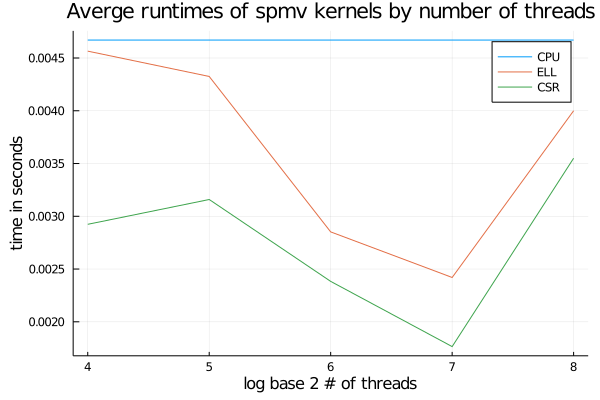
\includegraphics[scale=.5]{thread_runtime.png}
\end{figure}

\end{document}
